\section{Модифицированная задача}

\subsection{Постановка задачи}
\par Пусть, как и прежде, $L$ -- непустое конечное множество, называемое \textbf{множеством меток}. Пусть $G(V, E)$, $G'(V', E')$ -- ориентированные графы. Кроме того, будем полагать, что граф $G'$ -- связный. Для удобства дальнейшего изложения будем называть граф $G$ архивным графом, граф $G'$ -- графом-паттерном, или шаблонным графом.

Введём отображения $l : V \to L$, $l' : V' \to L$, сопоставляющие вершинам архивного и шаблонного графов соответствующие метки. Никаких дополнительных требований на эти отображения мы уже не накладываем.

Пусть также $\mathcal{X}$ -- это непустое (возможно, бесконечное) множество \textbf{(множество характеристик)} с заданным на нём бинарным отношением $\rho:\mathcal{X} \times \mathcal{X} \to \{0, 1\}$

Мы вводим множество характеристик для того, чтобы, например, работать со взвешенными графами. Действительно, если положить 

\[\mathcal{X} = \mathbb{R},\]
\[\rho(x, y) = \begin{cases}
1, & |x - y| < \varepsilon \\
0, & |x - y| \ge \varepsilon
\end{cases}, \varepsilon > 0,\]

мы получим отношение $\rho$, заданное, как отношение <<примерного равенства>>. Его мы и будем использовать для сравнения весов дуг архивного графа и графа-паттерна.

Введём также <<помечающие отображения>> для дуг графа: $\chi : E \to \mathcal{X}$, $\chi' : E' \to \mathcal{X}$.

Несколько изменится и определение совпадения.

\begin{defn}
	Взвешенным совпадением на графе $G$ будем называть частичный подграф $\widehat{G}(\widehat{V}, \widehat{E})$ графа $G$ такой, что:
	\begin{enumerate}
		\item Существует биективное отображение $m_{\widehat{G}}: V' \to \widehat{V}$.
		\item $\forall v' \in V': l'(v') = l(m_{\widehat{G}}(v'))$
		\item $\forall e' = (v^{\prime}_1, v^{\prime}_2) \in E': \rho(\chi'(e'), \chi((m_{\widehat{G}}(v^{\prime}_1), m_{\widehat{G}}(v^{\prime}_2)))) = 1$
		\item $\forall (v^{\prime}_1, v^{\prime}_2) \in E': (m_{\widehat{G}}(v^{\prime}_1), m_{\widehat{G}}(v^{\prime}_2)) \in E$
	\end{enumerate}
\end{defn} 

Пусть существует некоторое взвешенное совпадение  $\widehat{G}(\widehat{V}, \widehat{E})$ на графе $G$ такое, что есть вершина $v \in V : v \in \widehat{V}$. Тогда вершину $v$ будем называть подходящей паттерну $G'$ по взвешенному совпадению $\widehat{G}$, или истинным кандидатом, иначе -- неподходящей. В случае, если вершина $v$ подходит паттерну $G'$ по взвешенному совпадению $\widehat{G}$, вершину $v' = m_{\widehat{G}}^{-1}(v) \in  V'$ назовём соответствующей вершине $v$, а вершину $v$ -- соответствующей вершине $v'$.

Рассмотрим задачу нахождения соответствующих вершин для каждой из вершин графа $G'$. В следующих двух разделах описаны модификации алгоритмов из статьи \cite{patmat}, решающие задачу в такой постановке. В разделе \ref{ssec:recalg} описан алгоритм, восстанавливающий взвешенные совпадения по найденным соответствующим вершинам.

\subsection{Измененный алгоритм исключения по локальным условиям}

Пусть $T = 2^{V}$ -- все подмножества множества вершин графа-паттерна. Построим отображение $f_0 : V' \to T$, заданное следующим:
\begin{equation}
f_0(v') \{v \in V | l(v) = l'(v')\} .
\end{equation}

В отличие от приведённого в предыдущей части работы, это отображение сопоставляет каждой вершине графа-паттерна вершину какое-то подмножество вершин архивного графа. Также это отображение является истинно многозначным, т.е. элементами его образа являются, в общем случае, не только 0- и 1-элементные подмножества множества $V$. 

В связи с изменением области значений и определения введённого отображения $f_0$ следует изменить и операцию $Exclude$. Пусть $f_1, f_2 : V' \to 2^{V}$. Обозначим $f_2 = Exclude(f_1, v_0 (\in V), v^{\prime}_0 (\in V'))$, если выполнено следующее:
\begin{enumerate}
	\item $\forall v' \ne v^{\prime}_0 \in V': f_1(v') = f_2(v')$.
	\item $v_0 \notin f_2(v^{\prime}_0)$.
	\item $\{v_0\} \cup f_2(v^{\prime}_0) = f_1(v^{\prime}_0)$
\end{enumerate}

Ниже приведён изменённый алгоритм исключения по локальным условиям. Он принимает те же самые графы, но входное и выходное отображение имеют другие области определения и значений. Общая идея алгоритма сохраняется.

\begin{algorithm}[H]
	\Large
	\KwIn{графы $G(V, E)$, $G'(V', E')$, отображение $f_0 : V' \to T$, число итераций $N$}
	\KwOut{измененённое отображение $f_K$}
	\Begin(MLCCE){
		$K := 0$
		
		$F_0 := f_0$
		
		\For{$i = 1, 2, .., N$}{
			\For{$(q_0, q) \in E'$}
			{
				\For{$v_0 \in f(q_0)$}{
					$flag := False$
					
					\For{$v \in \Gamma(v_0)$}{
						\If{$v \in f_K(q)$}{
							\If{$\rho(\chi(v_0, v), \chi'(q_0, q)) = 1$}{
								$flag := True$
							}
						}
					}
				
					\If{$flag = False$}{
						$f_{K+1} := Exclude(f_{K}, v_0, q_0)$
						
						$K := K + 1$
					}
				}
				\For{$v \in f(q)$}{
					$flag := False$
					
					\For{$v_0 \in \Gamma^{-1}(v)$}{
						\If{$v_0 \in f_K(q_0)$}{
							\If{$\rho(\chi(v_0, v), \chi'(q_0, q)) = 1$}{
								$flag := True$
							}
						}
					}
					
					\If{$flag = False$}{
						$f_{K+1} := Exclude(f_{K}, v, q)$
						
						$K := K + 1$
					}
				}
			}
			
			$F_i := f_K$
		}
		\Return{$f_N$}
	}
	
	\caption{Измененный алгоритм исключения по локальным условиям}
	\label{alg:MLCCE}
\end{algorithm}

Алгоритм $MLCCE$ полностью берёт идею алгоритма, изложенного выше, а потому его корректность прямо вытекает из корректности вышеизложенного алгоритма. Мы лишь добавили пару циклов для того, чтобы обрабатывать многозначность, а также ориентированность графов $G$ и $G'$.

Сложность приведённого алгоритма, очевидно, выше сложности алгоритма $LCCE$. Оценим её на одной итерации. Поскольку $|\Gamma(v_0)|, |\Gamma^{-1}(v_0)| \le |V|$, то
\[T = \sum\limits_{(q_0, q) \in E'}  |f_i(q_0)| \cdot |V| = \sum\limits_{q_0 \in V'}  |\Gamma(q_0)|\cdot|f_i(q_0)|\cdot |V| \le \]

В худшем случае $f(q_0) = |V|$, имеем:
\[ \le |E'|\cdot|V|^2. \]

Таким образом, $T = O(|E'|\cdot|V|^2)$

Худший случай, однако, реализуется, только если задача поиска паттерна вырождается в задачу изоморфизма. Для реальных задач алгоритм $MLCCE$ работает достаточно быстро, за несколько итераций уменьшая число кандидатов на несколько порядков.

Заметим, однако, что в некоторых случаях даже на бесконтурных графах алгоритм \ref{alg:MLCCE} может не исключать некоторые вершины из списка кандидатов, несмотря на то, что они не являются истинным кандидатами. Простейший пример приведён на рисунке \ref{fig:fail}. В таких случаях можно, во-первых, применить фильтрацию по степеням вершин, а во-вторых, воспользоваться алгоритмом поиска взвешенного совпадения из последнего раздела данной работы.

\begin{figure}[H]
	\caption{Пример графов $G$ и $G'$, для которых алгоритм $MLCCE$ не исключает неистинных кандидатов}
	\centering
	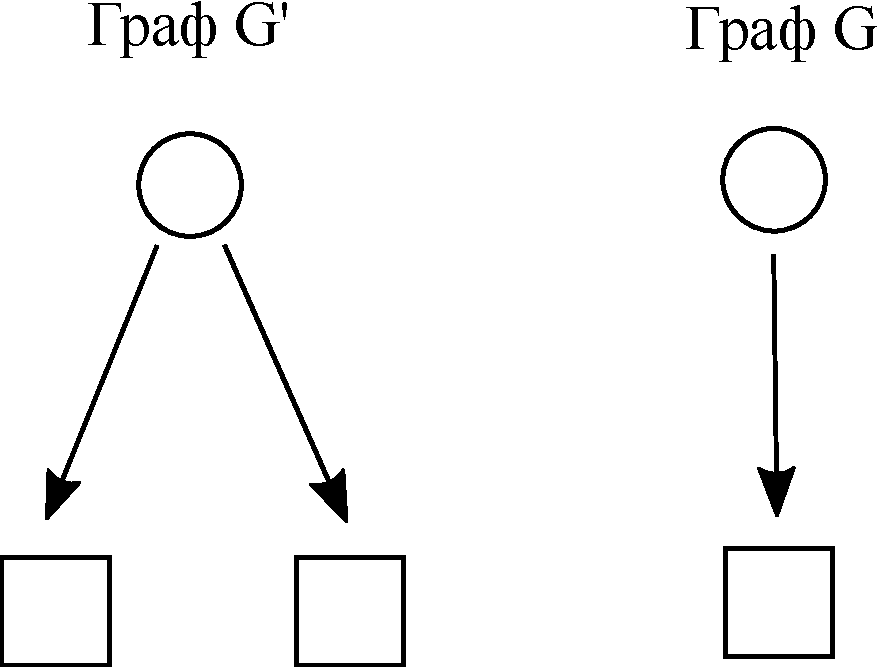
\includegraphics[width=0.5\textwidth]{failgraphs}
	\label{fig:fail}
\end{figure}

\subsection{Измененный алгоритм проверки контуров}

Для корректного исключения кандидатов на графах с контурами также был модифицирован алгоритм проверки контуров. 

Данный алгоритм проверяет на истинность кандидатов $\widehat{v}_0$ всех вершин $v_0^{\prime}$ графа-паттерна, в которых начинается какой-то контур $\mathcal{C}_0$. Для этого на каждой итерации цикла по дугам контура $\mathcal{C}_0$ создаётся множество вершин $\mathcal{B}$, в которое добавляются те вершины, которые соединены с вершинами множества $\mathcal{A}$ подходящими по характеристике дугами. Также проверяется, что концы этих дуг графа $G$ являются кандидатами для соответствующих концов рассматриваемой на текущей итерации дуги контура $\mathcal{C}_0$. После этого множеству $\mathcal{A}$ присваивается множество $\mathcal{B}$. Таким образом, после $s$ итераций цикла по дугам множество $\mathcal{A}$ содержит все вершины, на которые оканчиваются пути длины $s$, начинающиеся в вершине $\widehat{v}_0$ и являющиеся возможными взвешенными соответствиями пути, состоящего из первых $s$ дуг контура $\mathcal{C}_0$. Отдельно обрабатывается случай последней дуги контура, конец которой должен совпадать с началом первой дуги.

Псевдокод изменённого алгоритма проверки контуров приведён ниже (алгоритм \ref{alg:MCCE}).

\begin{algorithm}[H]
	\Large
	\KwIn{графы $G(V, E)$, $G'(V', E')$, отображение $f_0 : V' \to T$}
	\KwOut{измененённое отображение $f_N$}
	\Begin(MCCE){
		$K := 0$
		
		\ForEach{$\mathcal{C}_0 \in \mathcal{K}_0$}{
			Пусть $(v_0^{\prime}, v_1^{\prime})$ -- первая дуга контура $\mathcal{C}_0$.
			
			\For{$\widehat{v}_0 \in f_K(v_0^{\prime})$}{
				$\mathcal{A} := \{\widehat{v}_0\}$
				
				\For{$s = 1, 2, ..., |\mathcal{C}_0|$}{
					Пусть $(q_0, q_1)$ -- $s$-я дуга контура $\mathcal{C}_0$.
					
					$\mathcal{B} := \emptyset$
					
					\ForEach{$v_0 \in \mathcal{A}$}{
						\ForEach{$v_1 \in f_K(q_1)$}{
							$flag := False$
							
							\If{$v_1 \in \Gamma(v_0)$}{
								\If{$s \ne |\mathcal{C}_0| \lor \widehat{v}_0 = v_1$}{
									\If{$\rho(\chi(v_0, v_1), \chi'(q_0, q_1)) = 1$}{
										$flag := True$
									}
								}
							}
						
							\If{$flag = True$}{
								$\mathcal{B} := \mathcal{B} \cup \{v_1\}$
							}
						}
					}
					
					$\mathcal{A} := \mathcal{B}$ 
				}
			
				\If{$\widehat{v}_0 \notin \mathcal{A}$}{					
					$f_{K+1} := Exclude(f_{K}, \widehat{v}_0, v_0^{\prime})$
						
					$K := K + 1$
				}
			}
		}
		\Return{$f_N$}
	}
	
	\caption{Изменённый алгоритм проверки контуров}
	\label{alg:MCCE}
\end{algorithm}

Поскольку для любой вершины $v' \in V' \quad |f(v')| \le |V|$, а также $|\mathcal{A}| \le |V|$ и $|\mathcal{C}| \le E'$, сложность измененного алгоритма можно грубо оценить как $T = O(|\mathcal{K}_0| \cdot |V|^3 \cdot |E'|)$.

\subsection{Рекурсивный алгоритм выделения взвешенного совпадения} \label{ssec:recalg}

Общий алгоритм без каких-либо изменений переносится с уже введённого выше (алгоритм \ref{alg:EE}). Разница лишь в том, что передаваемое ему отображение формируется так, как указано выше в этом разделе.

Таким образом, построен алгоритм, решающий гораздо более общую задачу. Однако полученное после его работы отображение $f_N$ не может использоваться непосредственно -- необходимо ещё выделить взвешенные совпадения на графе $G$. Для решения этой задачи будем использовать описанный ниже алгоритм.

Для восстановления взвешенных совпадений по полученному отображению $f$ был разработан следующий метод:

\begin{enumerate}
	\item Преобразовать граф-паттерн $G'$ к особому виду, снабдив его дополнительной информацией, получив таким образом граф $G_0$.
	\item Положить $i := 0$.
	\item Пока граф $G_i$ имеет более одной вершины:
	\begin{enumerate}
		\item Выполнить на графе $G_i$ обход в ширину с окраской.
		\item Выделить подграфы графа $G_i$ с вершинами одного цвета.
		\item На каждом выделенном подграфе $G_i^j(V_i^j, E_i^j)$ построить все возможные соответствия между его вершинами и вершинами архивного графа.
		\item Сформировать новый граф $G_{i+1}$, взяв в качестве вершин подграфы $G_i^j$, а в качестве дуг -- дуги, вершины которых принадлежат сразу нескольким подграфам.
		\item Положить $i := i + 1$.
	\end{enumerate}
\end{enumerate}

Рассмотрим подробнее каждый из этих пунктов.

Преобразование графа $G'$ выполняется следующим образом: каждая его вершина $v'$ получает как характеристику список соответствий $\xi(v')$. Каждый список соответствий состоит из кортежей, элементами которых являются пары вида $(q_0, v_0)$, означающих, что вершине $q_0$ графа-паттерна соответствует вершина $v_0$ архивного графа. Таким образом, изначально для каждой вершины $v' \in V'$:
\[\xi(v') = [((v', v_1)), ..., ((v', v_L))], v_1, ..., v_L \in f(v_L).\]

Граф $G'$ со списками соответствий $\xi$ будем считать начальным графом для алгоритма выделения взвешенных соответствий и обозначать $G_0$.

Опишем алгоритм поиска в ширину с окраской, необходимый для решения задачи разбиения графа $G_i$ на подграфы. Процедура $BFS_C$, приведённая ниже (алгоритм \ref{alg:bfsc}), окрашивает максимум $N$ вершин графа $G$ в порядке обхода в ширину, начиная со стартовой вершины $s$.

\begin{algorithm}[H]
	\Large
	\KwIn{граф $G(V, E)$, вершина $s \in V$, отображение $c : V \to \mathbb{Z}_{+}$, цвет $i$, лимит вершин $N$}
	\KwOut{измененённое отображение $c$}
	\Begin($BFS_C$){
		$n := 0$
		
		Пусть $Q$ -- пустая очередь
		
		Добавить $s$ в $Q$
		
		\While{очередь $Q$ не пуста и $n < N$}{
			Извлечь вершину $v$ из очереди $Q$.
			
			$c(s) := i$
			
			$n := n + 1$
			
			\ForAll{$v_0 \in \Gamma(v)$}{
				\If{$c(v_0) \ne 0$}{
					Добавить вершину $v_0$ в очередь $Q$.
				}
			}
		}
		
		\Return{$c$}
	}
	
	\caption{Обход в ширину с окраской}
	\label{alg:bfsc}
\end{algorithm}

Процедуру \ref{alg:bfsc} используем в общем алгоритме окраски графа \ref{alg:cbfsc}.

\begin{algorithm}[H]
	\Large
	\KwIn{граф $G(V, E)$, лимит вершин $N$}
	\KwOut{окрашивающее отображение $c$, количество цветов $K$}
	\Begin($BFS Coloring$){
		
		\For{$v \in V$}{
			$c(v) := 0$
		}
		
		$i := 0$
		
		\While{$\exists v : c(v) = 0$}{
			Пусть вершина $v$ такова, что $c(v) = 0$
			
			$i := i + 1$
			
			$c := BFS_C(G, v, c, i, N)$
		}
		
		\Return{$c, i$}
	}
	
	\caption{Общий алгоритм ограски графа}
	\label{alg:cbfsc}
\end{algorithm}

После окраски по тем вершинам графа $G_i$, для которых алгоритм \ref{alg:cbfsc} определил одинаковые цвета, выделим подграфы $G_i^1, ..., G_i^K$.

В каждом выделенном подграфе отыщем все взвешенные совпадения, для чего воспользуемся алгоритмом \ref{alg:findall}

\begin{algorithm}[H]
	\Large
	\KwIn{подграф $G_i^j(V_i^j, E_i^j)$, списки соответствий $\xi$}
	\KwOut{новый список соответствий $\xi_i^j$}
	\Begin($Matching$){
		
		$\xi_i^j := []$
		
		\ForAll{конкатенаций всевозможных сочетаний кортежей в списках $\xi(v')$, $v' \in V_i^j$}{
			Пусть $((q_0, v_0), ..., (q_M, v_M))$ -- соответствующая конкатенация.
			
			\If{среди вершин $v_0, ..., v_M$ есть одинаковые}{ 
				Перейти к следующей итерации
			}
			
			$flag := True$
			
			\ForAll{дуг $(q_s, q_r)$ графа $G'$, концами которых являются вершины $q_0$, ...,  $q_M$}
			{
				\If{$(v_s, v_r) \notin E \lor \rho(\chi(q_s, q_r), \chi'(v_s, v_r)) = 0$}{
					$flag := False$
				}
			}
			
			\If{$flag = True$}{
				Добавить соответствие $((q_0, v_0), ..., (q_M, v_M))$ в список $\xi_i^j$
			}
		}
		
		\Return{список $\xi_i^j$}
	}
	
	\caption{Алгоритм поиска взвешенных совпадений для подграфа}
	\label{alg:findall}
\end{algorithm}

Таким образом, для каждого полученного на этапе раскраски подграфа $G_i^j$ будет получен единственный список соответствий $\xi_i^j$. После этого нам остаётся описать переход к следующей итерации цикла.

Для следующей итерации мы строим граф $G_{i+1}(V_{i+1}, E_{i+1})$, для которого:
\[V_{i+1} = \{G_i^1, ..., G_i^K\}, \]
\[E_{i+1} = \{(G_i^{j'}, G_i^{j''}) | \exists v' \in V_i^{j'} \quad \exists v'' \in V_i^{j''} \quad \exists (v', v'') \in E_i \}, \]
\[\xi(G_i^j) = \xi_i^j, j = 1, 2, ..., K\]

В силу связности графа $G'$ алгоритм завершается для любого лимита вершин $N > 1$. Поскольку выполняется сравнение характеристик всех рёбер (а по построению графа $G_0$ -- и меток вершин), список соответствий $\xi(v^{*})$, где $v^{*}$ -- единственная вершина графа, на котором произошёл выход из цикла, содержит списки точных вершинных соответствий, по каждому из которых можно восстановить взвешенное соответствие как подграф графа $G$. Действительно, если $((q_0, v_0), (q_1, v_1), ..., (q_l, v_l))$ -- некое вершинное совпадение, то граф $\widehat{G}(\widehat{V}, \widehat{E})$, где

\[\widehat{V} = \{v_0, v_1, ..., v_l\},\]
\[\widehat{E} = \{(v_i, v_j) | (q_i, q_j) \in E'\},\]
есть взвешенное совпадение на архивном графе $G$.